\begin{frame}
\frametitle{Modelo de cámara pinhole}

\pnote{* Lo anterior asume que el origen de coordenadas del plano de la imagen se encuentra en el punto principal. En la práctica, esto no siempre se cumple.}

\pnote{* Explicar representación en coordenadas homogéneas.}

Siendo $\begin{bmatrix}c_{u} & c_{v}\end{bmatrix}^{\top}$ la posición del punto principal.
\begin{equation}
\begin{bmatrix}x\\
y\\
z
\end{bmatrix}\longmapsto\begin{bmatrix}fx/z+c_{u}\\
fy/z+c_{v}
\end{bmatrix}
\end{equation}

En coordenadas homogéneas:

\begin{equation}
\begin{bmatrix}x\\
y\\
z\\
1
\end{bmatrix}\longmapsto\begin{bmatrix}fx+zc_{u}\\
fy+zc_{v}\\
z
\end{bmatrix}=\begin{bmatrix}f &  & c_{u} & 0\\
 & f & c_{v} & 0\\
 &  & 1 & 0
\end{bmatrix}\begin{bmatrix}x\\
y\\
z\\
1
\end{bmatrix}
\end{equation}

\begin{block}{Matriz de calibración intrínseca $\intrinsicMatrix$}
\begin{equation}
\intrinsicMatrix=\begin{bmatrix}f & 0 & c_{u}\\
0 & f & c_{v}\\
0 & 0 & 1
\end{bmatrix}
\end{equation}
\begin{equation}
\homo{\imagePoint}=\intrinsicMatrix\begin{bmatrix}\vec{{I}} & \vec{{0}}\end{bmatrix}\homo{\point}
\end{equation}
\end{block}

\end{frame}


\begin{frame}
\frametitle{Modelo de cámara pinhole}

\pnote{* Las ecuaciones anteriores deben extenderse agregando la transformación existente entre los sistemas de coordenadas de la cámara y el mundo.}

\pnote{* R es una matriz de rotación y t un vector de traslación.}

Puntos expresados en referencia al sistema de coordenadas del \textit{mundo}. La cámara no se encuentra necesariamente ubicada en el centro de este.

\begin{figure}[!htb]
	\centering
	\subfloat[]{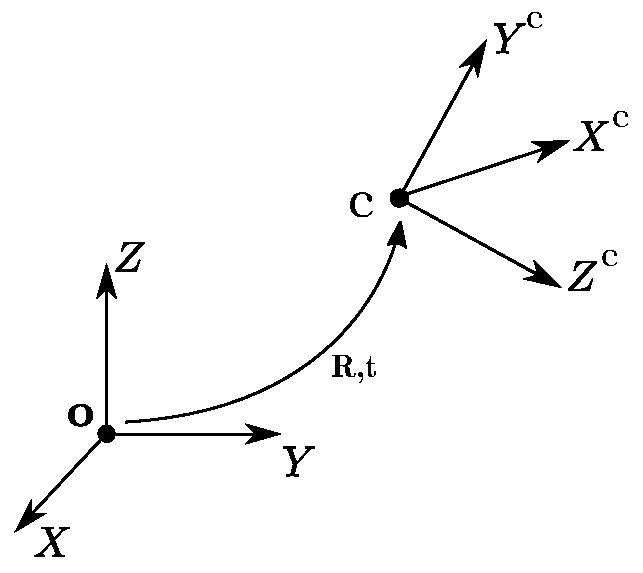
\includegraphics[width=0.4\columnwidth]{./cameras/camera_coord_system.pdf}}%
	\hfill
\end{figure}

\begin{block}{}
\begin{equation}
\homoCameraPoint=\begin{bmatrix}\rotation & \translation\\
0 & 1
\end{bmatrix}\begin{bmatrix}x\\
y\\
z\\
1
\end{bmatrix}=\seMatrix^{\mathrm{c}\mathrm{w}}\homoWorldPoint\;.
\end{equation}
\end{block}

\end{frame}


\begin{frame}
\frametitle{Modelo de cámara pinhole}

De esta manera, es posible proyectar cualquier punto 3D
$\homoWorldPoint$ en el sistema de coordenadas del mundo al correspondiente
punto $\homo{\imagePoint}$ en el plano de la imagen mediante:

\begin{block}{Matriz de proyección \textmd{$\projectionMatrix$}}
\begin{equation}
\projectionMatrix=\intrinsicMatrix\begin{bmatrix}\rotation & \translation\end{bmatrix}
\end{equation}
\begin{equation}
\homo{\imagePoint}=\projectionMatrix\homoWorldPoint
\end{equation}
\end{block}

\end{frame}


\begin{frame}
\frametitle{Modelo de cámara estéreo}

\begin{block}{Geometría epipolar}

\pnote{* La geometría proyectiva intrínseca entre dos cámaras es conocida como geometría epipolar.}

\pnote{* Esta es independiente de la escena observada y depende únicamente de los parámetros internos geometría epipolar y las posiciones relativas de las cámaras involucradas.}

Cualquier punto 3D $\point$ en el espacio, sus proyecciones $\imagePoint$ y $\imagePoint^{\prime}$ en los planos de las imágenes y los centros focales de las cámaras, pertenecen a un mismo plano $\vec{\pi}$.
De manera análoga, los rayos re-proyectados desde $\imagePoint$ y $\imagePoint^{\prime}$ se intersectan en $\point$, son coplanares y yacen sobre $\vec{\pi}$.
\end{block}

\begin{figure}[!htb]
	\centering
	\subfloat[]{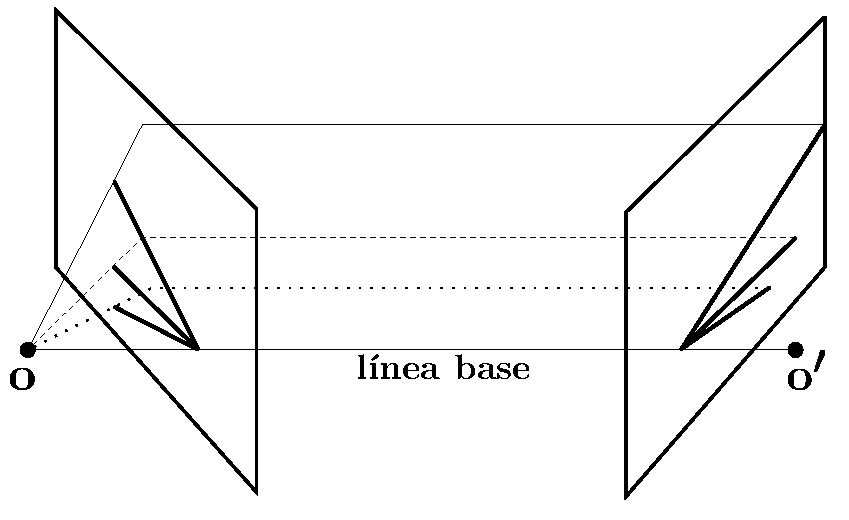
\includegraphics[width=0.5\columnwidth]{./cameras/pencil_of_planes.pdf}}%
	\hfill
	\centering
	\subfloat[]{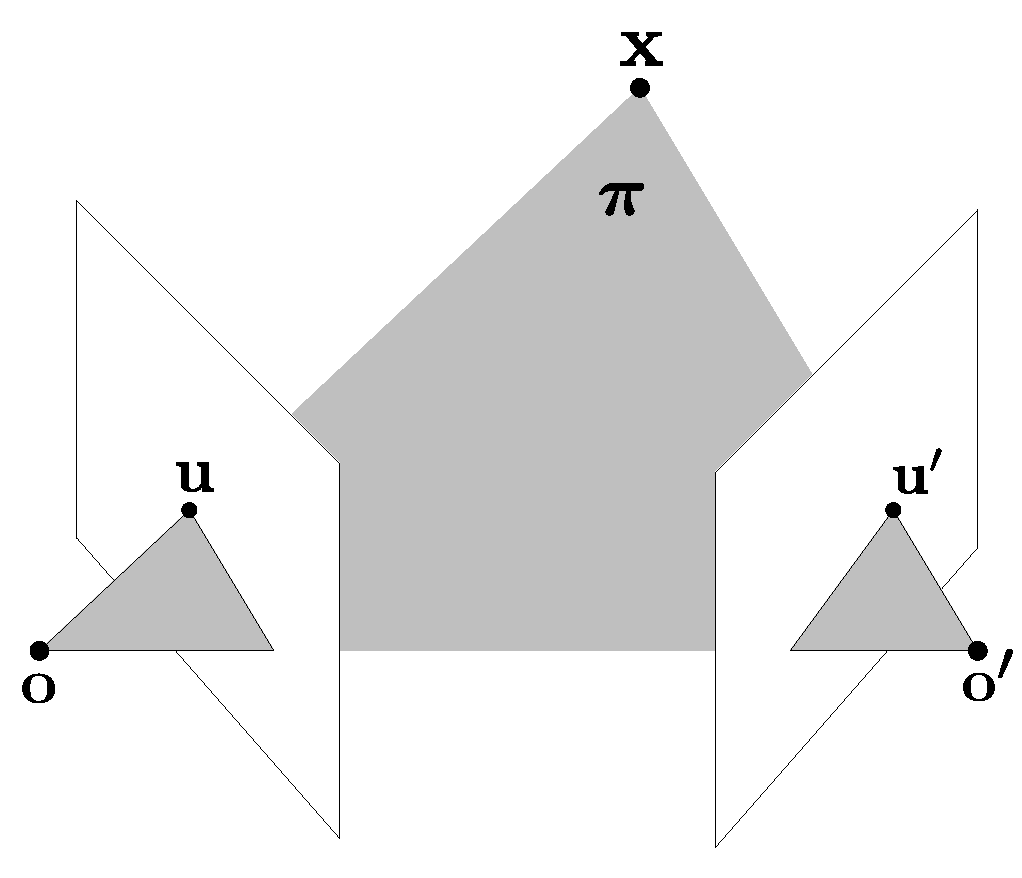
\includegraphics[width=0.5\columnwidth]{./cameras/epipolar_plane.pdf}}%
	\hfill
\end{figure}
\end{frame}


\begin{frame}
\frametitle{Modelo de cámara estéreo}

\pnote{* La búsqueda del correspondiente al punto u no necesita cubrir el plano de la imagen completo sino que puede restringirse a la línea epipolar l.}

\pnote{* La línea epipolar es generada por la proyección del rayo, re-proyectado desde u, sobre el plano focal de la segunda imagen.}

Búsqueda de correspondencias sobre la línea epipolar.

\begin{figure}[!htb]
	\centering
	\subfloat[]{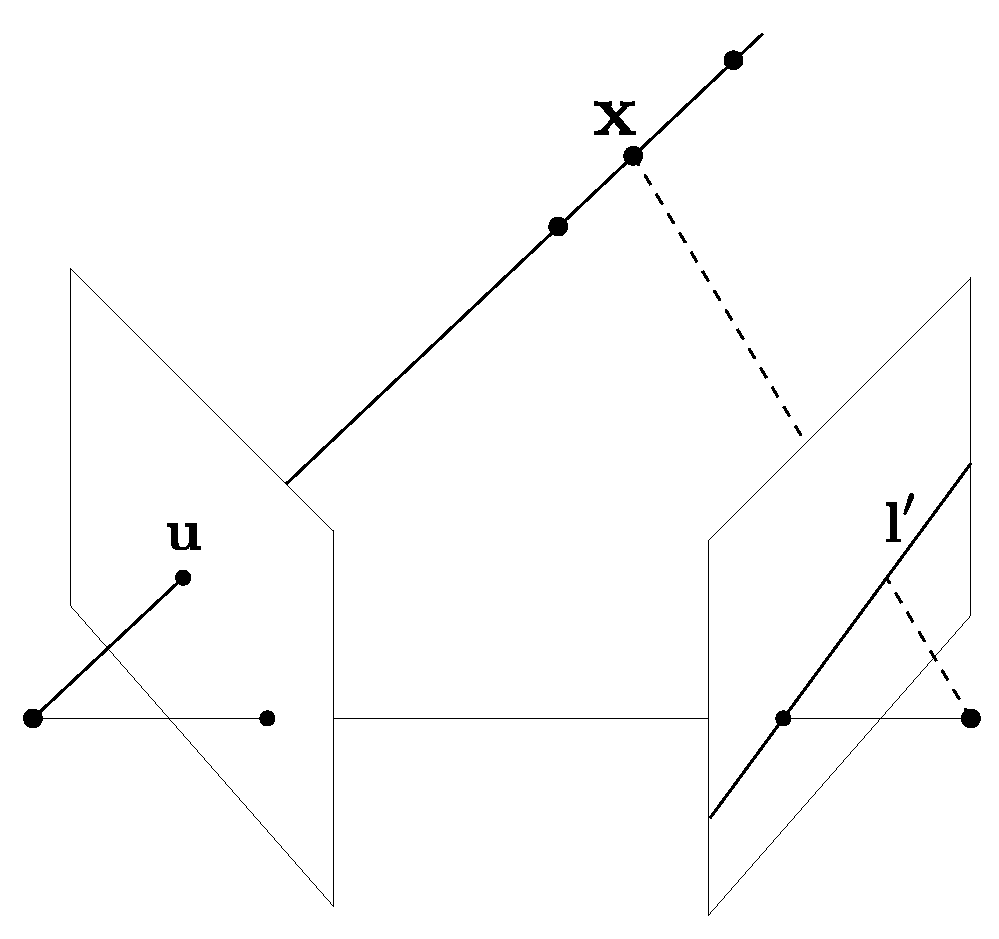
\includegraphics[width=0.5\columnwidth]{./cameras/epipolar_line.pdf}}%
	\hfill
\end{figure}
\end{frame}


\begin{frame}
\frametitle{Rectificación estéreo}

\pnote{* Luego de aplicar rectificación estéreo, la búsqueda de correspondencias entre las imágenes es reducida a una búsqueda unidimensional, sobre la misma fila.}

\begin{itemize}
\item Proyectar el par de imágenes estéreo sobre un plano de imagen común.
\item Los puntos correspondientes se encuentren alineados en la misma fila.
\end{itemize}

\begin{figure}[!htb]
	\centering
	\subfloat[]{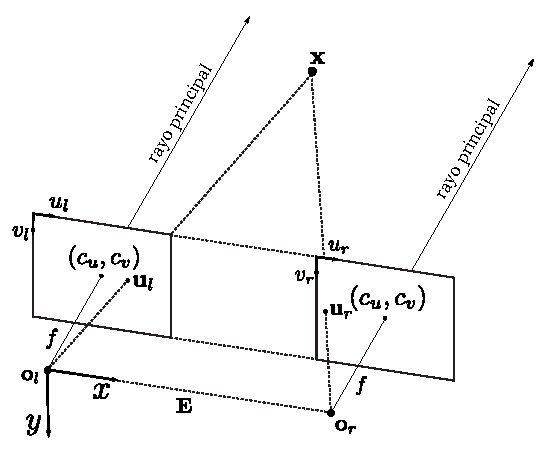
\includegraphics[width=0.6\columnwidth]{./cameras/stereo_rectification.pdf}}%
	\hfill
\end{figure}
\end{frame}


\begin{frame}
\frametitle{Rectificación estéreo}

\pnote{* Rectificación estéreo sobre un par de imágenes del Dataset Level 7 [32]. (a) Par de imágenes estéreo original provisto por la cámara estéreo.}
\pnote{* (b) El par de imágenes estéreo luego de ser rectificadas. Las líneas rojas asocian algunos puntos correspondientes entre ambas imágenes. Notar que estos puntos se encuentran en la misma fila en ambas imágenes.}

\begin{figure}[!htb]
	\centering
	\subfloat[]{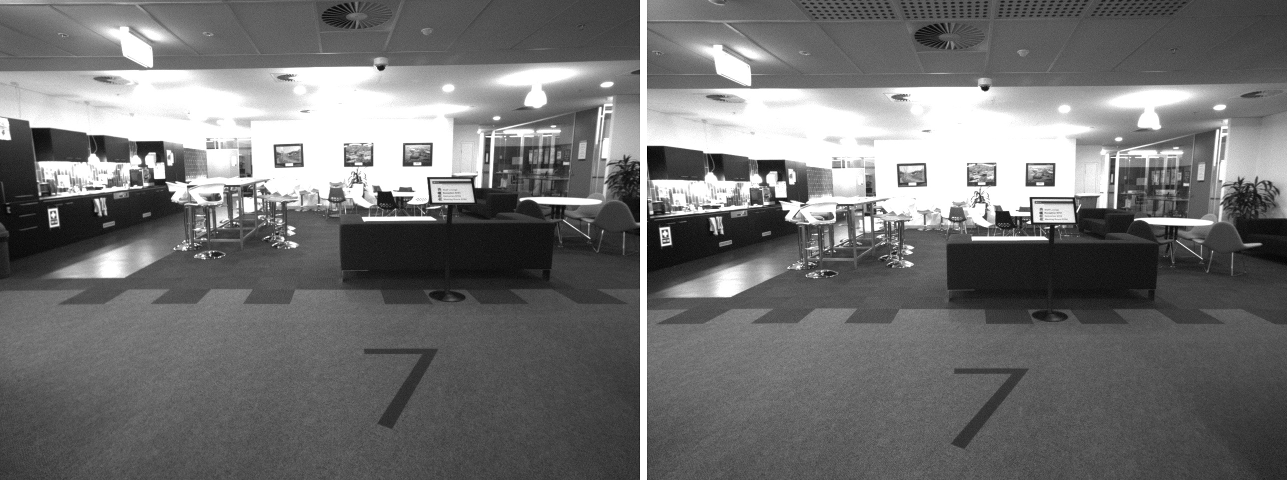
\includegraphics[width=0.6\columnwidth]{./cameras/no_rectified_stereo_images.png}}%
	\hfill
	\\
	\centering
	\subfloat[]{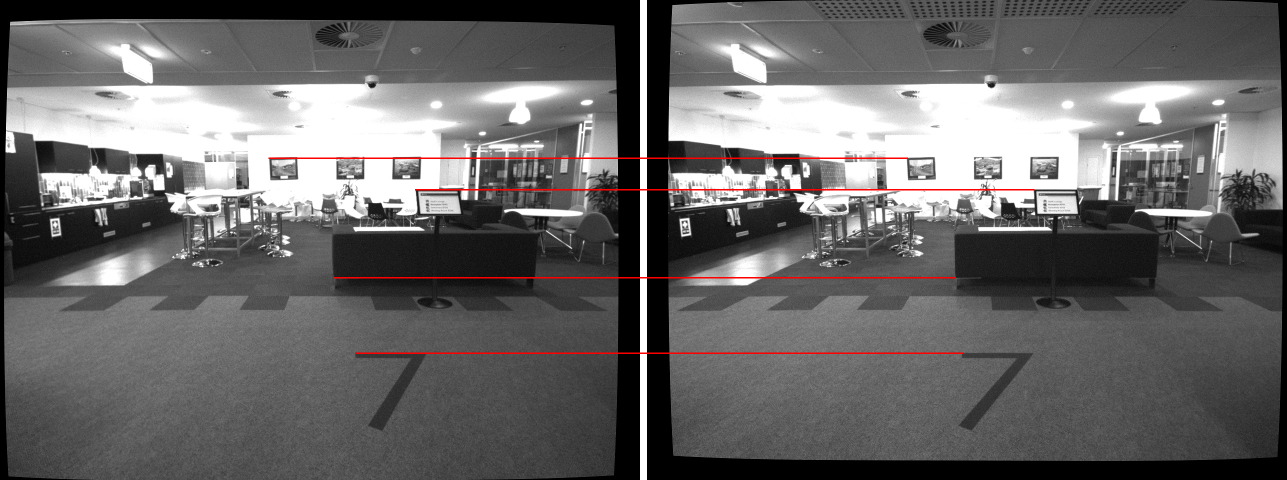
\includegraphics[width=0.6\columnwidth]{./cameras/rectified_stereo_images.png}}%
	\hfill
\end{figure}
\end{frame}


